% Created 2019-10-03 jue 19:35
% Intended LaTeX compiler: pdflatex
\documentclass[11pt]{article}
\usepackage[utf8]{inputenc}
\usepackage[T1]{fontenc}
\usepackage{graphicx}
\usepackage{grffile}
\usepackage{longtable}
\usepackage{wrapfig}
\usepackage{rotating}
\usepackage[normalem]{ulem}
\usepackage{amsmath}
\usepackage{textcomp}
\usepackage{amssymb}
\usepackage{capt-of}
\usepackage{hyperref}
\usepackage{listings}
\lstalias{ipython}{python}
\lstset{basicstyle=\small\ttfamily, frame=single}
\usepackage{bera}
\author{Invitado}
\date{\today}
\title{Árbol generador de menor costo}
\hypersetup{
 pdfauthor={Invitado},
 pdftitle={Árbol generador de menor costo},
 pdfkeywords={},
 pdfsubject={},
 pdfcreator={Emacs 25.2.2 (Org mode 9.2.1)}, 
 pdflang={English}}
\begin{document}

\maketitle

\section{Problema}
\label{sec:org33c88ae}

Supongamos que a cada arista de la gráfica completa \(K_{n}\) se le
asigna un valor ("peso"). Si a cada subgráfica le asignamos un peso
igual a la suma de los pesos de sus aristas, consideraremos el
problema de encontrar el árbol generador de menor peso.

\section{Algoritmo de Kruskal}
\label{sec:orga12921d}

El algoritmo de Kruskal consiste en escoger sucesivamente la arista
más barata de forma que no forme ciclo con la gráfica determinada por
las aristas escogidas previamente; si en algún momento existen varias
aristas que tienen el menor costo y no forman ciclos podemos escoger
cualquiera.

\section{Implementación en Python}
\label{sec:org7fc6dc9}

Primeramente vamos a importar las bibliotecas que vamos a utilizar.

\lstset{language=ipython,label= ,caption= ,captionpos=b,numbers=none}
\begin{lstlisting}
import networkx as nx
import matplotlib.pyplot as plt
from random import random as random
from scipy.spatial.distance import euclidean
\end{lstlisting}

A continuación definiremos una gráfica aleatoria con 10 vértices.

\lstset{language=ipython,label= ,caption= ,captionpos=b,numbers=none}
\begin{lstlisting}
g=nx.gnp_random_graph(10,0.2)
\end{lstlisting}

Veremos si nuestra gráfica aleatoria es un bosque.

\lstset{language=ipython,label= ,caption= ,captionpos=b,numbers=none}
\begin{lstlisting}
nx.is_forest(g), nx.is_connected(g)
\end{lstlisting}

\begin{verbatim}
(True, False)
\end{verbatim}

A continuación dibujaremos esta gráfica
\lstset{language=ipython,label= ,caption= ,captionpos=b,numbers=none}
\begin{lstlisting}
nx.draw(g, with_labels=True)
\end{lstlisting}

\begin{center}
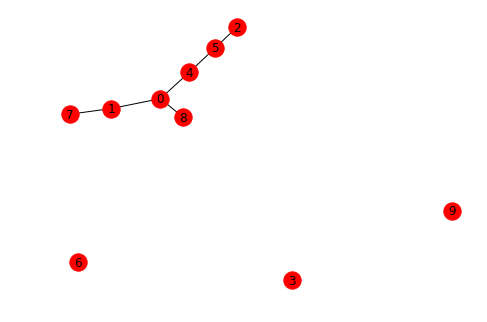
\includegraphics[width=.9\linewidth]{./obipy-resources/2747vnB.png}
\end{center}

Calcularemos las componentes conexas de esta gráfica:
\lstset{language=ipython,label= ,caption= ,captionpos=b,numbers=none}
\begin{lstlisting}
list(nx.connected_components(g))
\end{lstlisting}

\begin{verbatim}
[{0, 1, 2, 4, 5, 7, 8}, {3}, {6}, {9}]
\end{verbatim}

Veamos la componente que contiene al vértice 2.

\lstset{language=ipython,label= ,caption= ,captionpos=b,numbers=none}
\begin{lstlisting}
nx.node_connected_component(g,2)
\end{lstlisting}

\begin{verbatim}
{0, 1, 2, 4, 5, 7, 8}
\end{verbatim}

A continuación dibujaremos un árbol escogido aleatoriamente. 

\lstset{language=ipython,label= ,caption= ,captionpos=b,numbers=none}
\begin{lstlisting}
t=nx.random_tree(10)
nx.draw(t, with_labels=True)
\end{lstlisting}

\begin{center}
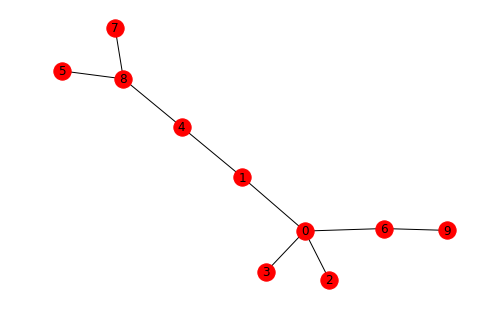
\includegraphics[width=.9\linewidth]{./obipy-resources/27478xH.png}
\end{center}

\section{Puntos en el plano}
\label{sec:org4b5391a}

Si tenemos dos listas de números de tamaño \texttt{n}, podemos dibujar \texttt{n} puntos en el plano,
las coordenadas \texttt{x} de la primera lista y las coordenadas \texttt{y} de la segunda.

\lstset{language=ipython,label= ,caption= ,captionpos=b,numbers=none}
\begin{lstlisting}
plt.plot([1,1,2],[1,2,3],'rx')
plt.axis([0,3,0,4])
plt.show()
\end{lstlisting}

\begin{center}
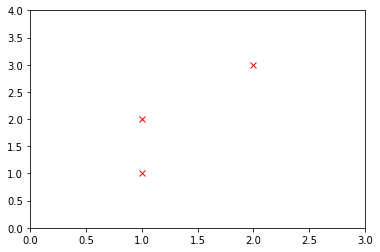
\includegraphics[width=.9\linewidth]{./obipy-resources/2747WGU.png}
\end{center}

Vamos a definir una función que dibuje \texttt{n} puntos en e plano aleatoriamente.

\lstset{language=ipython,label= ,caption= ,captionpos=b,numbers=none}
\begin{lstlisting}
def puntos_en_el_plano(n):
   listax=[]
   listay=[]
   for i in range(n):
       listax.append(random())
       listay.append(random())
   return listax, listay
\end{lstlisting}

\lstset{language=ipython,label= ,caption= ,captionpos=b,numbers=none}
\begin{lstlisting}
puntos=puntos_en_el_plano(50)
\end{lstlisting}

\lstset{language=ipython,label= ,caption= ,captionpos=b,numbers=none}
\begin{lstlisting}
plt.plot(puntos[0], puntos[1], 'ro')
plt.show()
\end{lstlisting}

\begin{center}
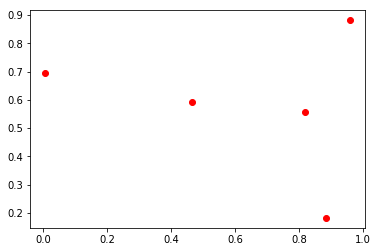
\includegraphics[width=.9\linewidth]{./obipy-resources/2747jQa.png}
\end{center}

Hagamos una función tal que a partir de dos listas, produzca el dibujo:

\lstset{language=ipython,label= ,caption= ,captionpos=b,numbers=none}
\begin{lstlisting}
def dibujo_puntos(listax, listay):
    plt.plot(listax, listay, 'ro')
    plt.axis([-0.1,1.1,-0.1,1.1])
    plt.gca().set_aspect('equal')
    plt.show()
\end{lstlisting}

\lstset{language=ipython,label= ,caption= ,captionpos=b,numbers=none}
\begin{lstlisting}
dibujo_puntos(*puntos)
\end{lstlisting}

\begin{center}
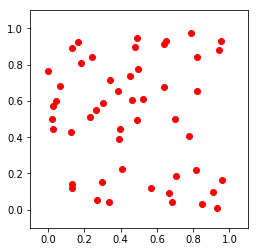
\includegraphics[width=.9\linewidth]{./obipy-resources/2747wag.png}
\end{center}
\end{document}